
\subsection{Client::ApplicationManager}
Package contenente le classi che si occupano della gestione delle applicazioni con le quali l'utente può interagire.\\ Vengono offerte funzionalità che permettono: \begin{itemize} \item la reazione a dei dati di risposta arrivati dal \file{Back-end}; \item la definizione di ciò che va a comporre una applicazione; \item il salvataggio dello stato di un'applicazione; \item il cambio di un'applicazione con un'altra. \end{itemize}



\subsection{Client::Logic}
Package contenente le classi che gestiscono la logica del client e che si occupano della comunicazione con il back-end.\\ Vengono offerte funzionalità che permettono: \begin{itemize} \item la reazione a dei dati arrivati come richiesta dal registratore vocale; \item il notificare alle classi interessate l'arrivo di dati dal \file{Back-end}. \end{itemize}
\begin{figure}[h] \centering 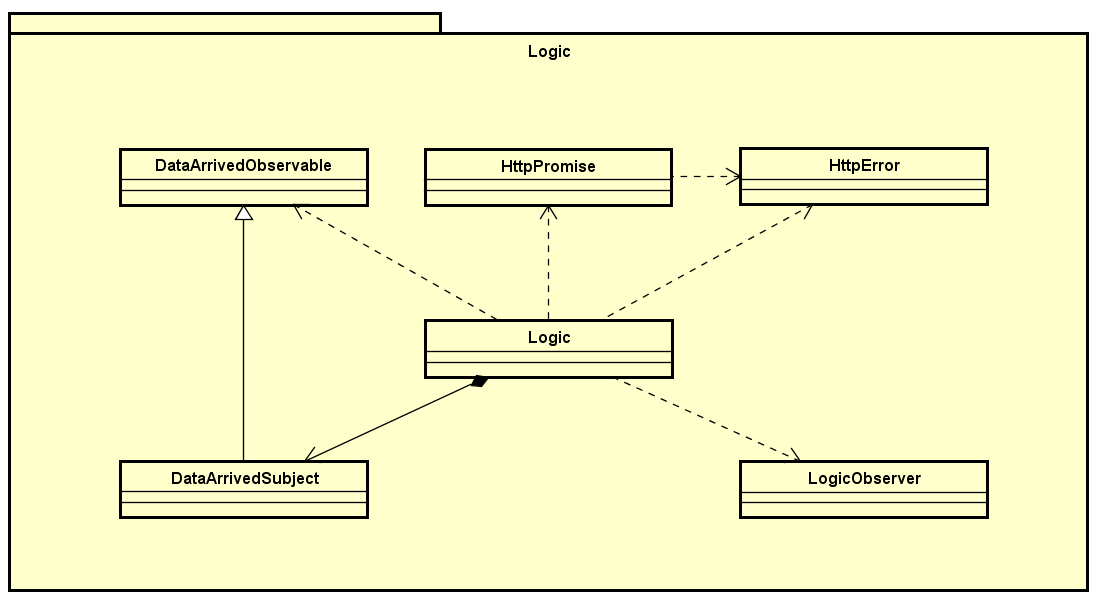
\includegraphics[width=\textwidth,height=\textheight,keepaspectratio]{images/diagrams/client/Client/Logic.png}
\caption{Package Client::Logic}
\end{figure}
\newpage


\subsection{Client::Recorder}
Package contenente le classi che realizzano la registrazione audio.\\ Vengono offerte funzionalità che permettono: \begin{itemize} \item la registrazione audio delle richieste espresse dall'utente; \item il notificare alle classi interessate la fine della registrazione audio di una richiesta dell'utente\file{Back-end}. \end{itemize}
\begin{figure}[h] \centering 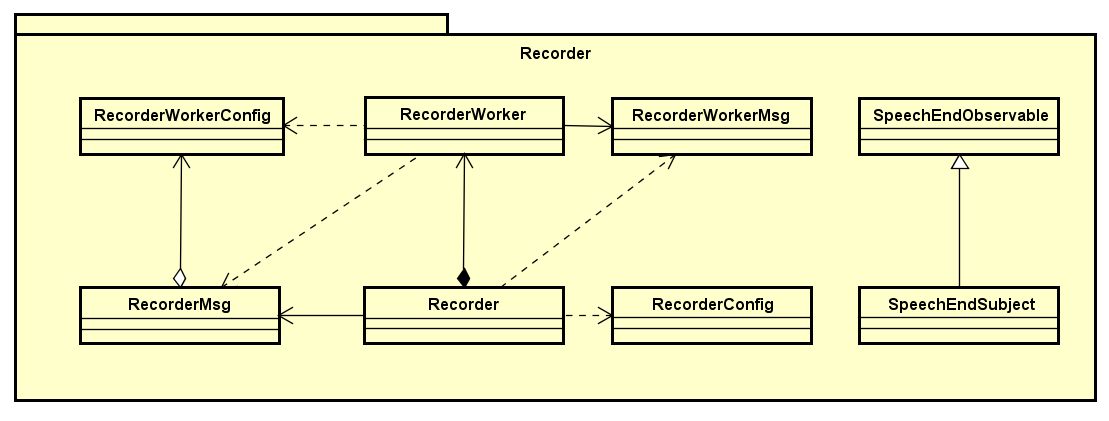
\includegraphics[width=\textwidth,height=\textheight,keepaspectratio]{images/diagrams/client/Client/Recorder.png}
\caption{Package Client::Recorder}
\end{figure}
\newpage


\subsection{Client::TTS}
Package contenente le componenti che realizzano il text to speech. Vengono offerte funzionalità che permettono: \begin{itemize} \item la reazione a dei dati arrivati come riposta dal \file{Back-end}; \item la riproduzione audio del testo fornito come risposta dall'assistente virtuale. \end{itemize}
\begin{figure}[h] \centering 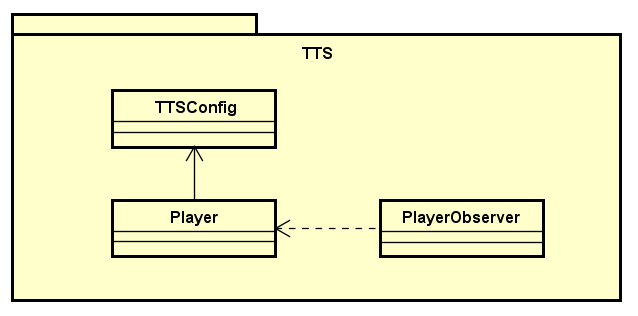
\includegraphics[width=\textwidth,height=\textheight,keepaspectratio]{images/diagrams/client/Client/TTS.png}
\caption{Package Client::TTS}
\end{figure}
\newpage


\subsection{Client::Utility}
Package contenente classi e interfacce, dallo scopo generico, utili ad altri package del client.
\begin{figure}[h] \centering 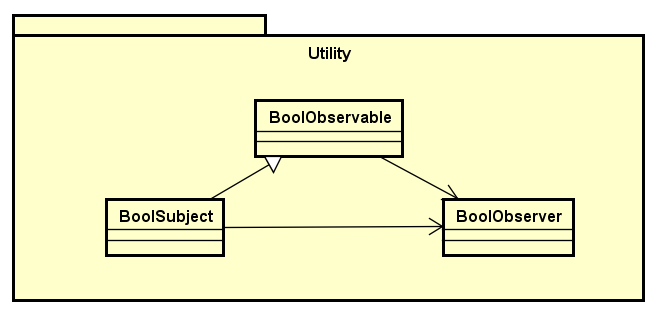
\includegraphics[width=\textwidth,height=\textheight,keepaspectratio]{images/diagrams/client/Client/Utility.png}
\caption{Package Client::Utility}
\end{figure}
\newpage